% preamble

\documentclass[letterpaper]{article}
\usepackage[utf8]{inputenc}
\usepackage{graphicx}
\usepackage{listings}
\usepackage{xcolor}

\definecolor{codegreen}{rgb}{0,0.6,0}
\definecolor{codegray}{rgb}{0.5,0.5,0.5}
\definecolor{codepurple}{rgb}{0.58,0,0.82}
\definecolor{backcolour}{rgb}{255,255,255}

\lstdefinestyle{mystyle}{
    backgroundcolor=\color{backcolour},   
    commentstyle=\color{codegreen},
    keywordstyle=\color{magenta},
    numberstyle=\tiny\color{codegray},
    stringstyle=\color{codepurple},
    basicstyle=\ttfamily\footnotesize,
    breakatwhitespace=false,         
    breaklines=true,                 
    captionpos=b,                    
    keepspaces=true,                 
    numbers=left,                    
    numbersep=5pt,                  
    showspaces=false,                
    showstringspaces=false,
    showtabs=false,                  
    tabsize=2
}

\lstset{style=mystyle}

\graphicspath{ {images/} }

\title{Using Citizen Science Species Occurrence Data to Study Biodiversity and Plan for the Future}
\author{Dylan Readel}
\date{February 2020}

% document

\begin{document}
\maketitle

\section*{Abstract}

Lorem ipsum dolor sit amet, consectetur adipiscing elit, sed do eiusmod tempor incididunt ut labore et dolore magna aliqua. Justo donec enim diam vulputate. Arcu vitae elementum curabitur vitae nunc sed velit dignissim sodales. Proin fermentum leo vel orci porta non pulvinar. Nascetur ridiculus mus mauris vitae ultricies leo integer. Facilisis magna etiam tempor orci eu. Vestibulum lorem sed risus ultricies. Euismod elementum nisi quis eleifend quam. Pulvinar sapien et ligula ullamcorper malesuada proin. Aenean pharetra magna ac placerat. Tempor id eu nisl nunc mi ipsum faucibus vitae. Et netus et malesuada fames ac turpis egestas sed. Duis ut diam quam nulla porttitor massa id neque aliquam. Euismod elementum nisi quis eleifend quam adipiscing vitae. Quam viverra orci sagittis eu volutpat odio.

\newpage

\tableofcontents
\listoffigures

\newpage

\section{Introduction}

\begin{itemize} \itemsep -0.15cm
	\item To understand the biodiversity of an area, it is important to know the species of that area and how many of each species are present.
	\item Understanding the biodiversity of an area is useful for preparing for the future. Urban areas like Los Angeles are novel ecosystems. The data collected by citizen scientists like the data available on iNaturalist is extremely useful for identifying what species live in urban areas. 
	\item For some species, seasonal distributions vary greatly. Database information can be utilized to understand how species come and go from an area over the course of a year. This seasonal distribution knowledge can be useful for identifying birds and insects that are still migrating through urban areas, or those that have changed courses to avoid the concrete jungles. 
	\item Literature regarding urban ecosystem planning, especially in the face of climate change, is crucial for understanding the importance of this project. Furthermore, literature regarding the use of historic species occurrence records highlights the significance of why identifying the species in an area is critical for future planning.
	
\end{itemize}

\section{Methods}

The following code is a function that is planned to be able to analyze any species occurrence dataset. These datasets can be retrieved from database websites like Global Biodiversity Information Facility (GBIF), Integrated Digitized Biocollections (iDigBio), iNaturalist, and Paleobiology Database (PBDB). The goal of the function is to help users understand the distribution of a desired taxonomic rank throughout the seasons in an area of interest. Furthermore, the function will supply the user with a CSV output file containing the counts of each taxon depending on the taxonomic rank specified by the user. If the user wants to know the count of every family or species in the dataset, then that can be completed with this function.

Regular expressions are utilized in an inner function of the code presented below. The regular expression, along with user input, is used to extract all the occurrences of a desired year and tell the user how many occurrences were from that year.

The function will eventually do much more with the datasets to provide the user with as much information that is necessary for researching the biodiversity of an area.

\newpage
\begin{lstlisting}[language=Python]
import pandas as pd
import datetime
import matplotlib.pyplot as plt
from datetime import datetime
from collections import defaultdict
import os
import csv

def taxonomic_dataset_analysis():
    '''
    This function is designed to read in a species occurrence dataset, analyze the data, and create useful outputs for understanding taxon occurrences 	throughout seasons. The function also outputs a CSV file that contains the counts of each unique taxon in the dataset in respect to the taxonomic rank specified by the user.
    
    -----------------------------------
    
    inputfile: a species occurrence CSV dataset
    date_col: the CSV column corresponding to the occurrence date
    '''
    
    inputfile = ''
    inputfile = input('Enter the dataset filename: ')
    
    # assert error for no filename specified
    assert len(inputfile) != 0, 'No filename entered.'
    # assert error that the filename specified is not a string
    assert type(inputfile) == str, 'Filename is not a string: %r' % inputfile

    print('Beginning seasonal occurrence analysis.')
    
    # read in the csv data file of species observations
    data = pd.read_csv(inputfile)
    
    # input for date column and assert that the date column exists within dataset
    date_col = ''
    date_col = input('Enter the observation date column header name: ')
    if date_col in data.columns:
        print('Column found!')
    assert date_col in data.columns, 'Date column header not found!'
        
    def seasonal_occurrences(data, date_col, inputfile):
        '''
        This inner function uses the occurrence dataset along with the date column specified to  create a histogram displaying specified taxonomic rank occurrences by season. The use of this is to visualize the seasonal distribution of species or to understand when people upload species observations to online databases such as iNaturalist.
        
        -------------------------------------
        
        User input is required to create the plot including the x-label, the y-label, and the title.
        '''

        # extract the dates column to a list
        dates = data[date_col].to_list()

        # create an empty list for dates that are separated using datetime
        dates_separated = list()

        # iterate through dates to separate them using datetime
        for i in dates:
            dates_separated.append(datetime.strptime(i, "%Y-%m-%d"))

        # create an empty list for observations by month
        months = list()

        # iterate through separated dates list to extract just the month as an integer
        for m in dates_separated:
            months.append(m.month)

        # create an empty list for observations by season
        observations_by_season = list()

        # iterate through each observation in the months list
        # by using an if statement for each season
        # if the month is in the season's numerical range
        # the season is appended to the observation_by_season list
        for x in months:
            if x in range(1, 4):
                observations_by_season.append('Winter')
            if x in range(4, 7):
                observations_by_season.append('Spring')
            if x in range(7, 10):
                observations_by_season.append('Summer')
            if x in range (10, 13):
                observations_by_season.append('Autumn')

        # create an empty default dictionary with integers
        # for the count of each observation by season
        season_counts = defaultdict(int)

        # iterate through seasons in observations_by_season list
        # add a count for each season to the season_counts dictionary
        for season in observations_by_season:
            season_counts[season] = season_counts[season] + 1

        x_label = ''
        x_label = input('Enter the label for the x-axis (something about seasons): ')
        y_label = ''
        y_label = input('Enter the label for the y-axis (something about number of occurrences): ')
        figtitle = ''
        figtitle = input('Enter the title for your figure: ')
        print("Sit tight, we're making the figure...")

        # plot a histogram of the season_counts dictionary
        plt.bar(season_counts.keys(), season_counts.values())

        # parameters for the figure
        plt.xlabel(x_label)
        plt.ylabel(y_label)
        plt.title(figtitle)
        plt.tight_layout()

        figure_save = ''
        figure_save = input('What do you want to call your figure save? ')
        plt.savefig(figure_save)
        print("Figure successfully saved!")

        print('Figure can be found at', os.path.abspath(figure_save))

        print('Now creating taxon count CSV file.')
    
    def taxon_counts(data, date_col, inputfile):
        ''' 
        This inner function is useful for ouputting a CSV file containing the counts of a desired taxonomic rank. For example, if the user specifies the family taxonomic rank, then a CSV file will be created that gives the counts of each family in the occurrence dataset.
        
        --------------------------------------
        
        This function is useful to understand the diversity of an area. An easy way to study the diversity of an area is to know what species are the most common or rare.
        '''
        
        # input for the desired taxonomic rank column
        # counts of each taxon placed in a dictionary
        taxon_col = ''
        taxon_col = input('Enter the taxon column header name: ')
        counts_dic = (data[taxon_col].value_counts()).to_dict()
        
        # input for the CSV save file
        outputcsv = ''
        outputcsv = input('What do you want to call your {} counts save?'.format(taxon_col))
    
        with open(outputcsv, 'w', newline = '') as csvfile:
            writer = csv.writer(csvfile)
            for species, counts in counts_dic.items():
                writer.writerow([species, counts])
                
        print('CSV file can be found at', os.path.abspath(outputcsv))
        
        # input for a user prompt of whether they want to know the count of a specific taxon
        answer = ''
        answer = input('Do you want to know the count of any specific taxon? Answer with Y or N.')
        answer = answer.upper()
        
        # answering yes brings user to another inner function
        if answer == 'Y':
            
            def counts_from_year(inputfile, date_col):
                '''
                
                This inner function utilizes a regular expression and user input to extract  occurrences from a user specified year and output the number of occurrences in total from that year. The regular expression searches the date column for all matches to the user's year.
                
                '''
                
                dates = []
                
                # reading in the data and appending the dates to a list
                with open(inputfile, 'r') as rf:
                    data = csv.DictReader(rf, delimiter = ',')
                    header = data.fieldnames
                    for dic in data:
                        dates.append(dic[date_col])
                
                # input for the desired year
                # generation of a regular expression based on the year input
                year = ''
                year = input('Enter the year you want the number of occurrences from: ')
                pre_regex = '[^-\d]*'
                regex = year + pre_regex
                charRe = re.compile(regex)

                year_specified = []
                year_counts = defaultdict(int)
                
                # appending each year match to a list
                for date in dates:
                    year_specified.append(charRe.match(date))
                
                # creating a dictionary with the key as the year and the value as the occurrences
                for obs in year_specified:
                    year_counts[obs] += 1

                # this is required because each year match gets added as a new key to the dictionary
                # but the None key in the dictionary has a value that is equal to every year that 
                # did not match the user input
                # the years that did not match is substracted from the total length of the dataset
                count = len(dates) - year_counts.get(None)

                print('The year {} had {} species observations.'.format(year, count))

            counts_from_year(inputfile, date_col)
        
        # if user answers no to prompt the analysis is completed
        if answer == 'N':
            
            print('Analysis completed.')
    
    seasonal_occurrences(data, date_col, inputfile)
    taxon_counts(data, date_col, inputfile)
    
taxonomic_dataset_analysis()

\end{lstlisting}

\newpage

The following code is intended to produce a map of the distribution of several species at once. Figure \ref{fig:map} shows the distribution of the three most common bird species in the LA River Watershed region presented on iNaturalist. The base layer can be changed for any region, but for this example a shapefile of LA County was used. The function is modular meaning any number of species or other taxon can be used and plotted. A new point variable can be created for each species or taxon. The function is designed to work with any dataset that includes latitude and longitude coordinates. The species are chosen using a grep command and extracting them from the dataset. This function is useful since a website like iNaturalist does not display different species as different point objects simultaneously. The map produced by this function allows the user to visualize how different species are spatially distributed across a region. The function can be modified to extract and plot different aspects of the datasets, as well. For example, instead of extracting and plotting species or other taxon, a user may want to extract iNaturalist user identification numbers and plot the distribution of them.

\begin{lstlisting}[language=R]
library(rgdal)
library(ggplot2)
library(dplyr)

dist_map <- function(filename) {
  
setwd('~/Documents/UCLA/UCLA Winter 2020/EEB C177/')
  
# read in bird occurrence data with coordinates
mapdata <- read.csv(filename, stringsAsFactors = FALSE)

# set a variable for each species that is to be plotted
# any number of variables can be assigned for the map
mapdata_mallard <- mapdata[grep('Anas platyrhynchos',
                                mapdata$taxon_species_name), ]
mapdata_dove <- mapdata[grep('Zenaida macroura',
                             mapdata$taxon_species_name), ]
mapdata_sparrow <- mapdata[grep('Passer domesticus',
                                mapdata$taxon_species_name), ]

# load in an LA County shapefile and set to a variable
county <- readOGR('DRP_COUNTY_BOUNDARY/DRP_COUNTY_BOUNDARY.shp', layer = 'DRP_COUNTY_BOUNDARY')

# useful for knowing how the county layer is being displayed
# for this shapefile, the projection used is NAD83
proj4string(county)

# find out what class the mapdata is
class(mapdata)

# creating a spatial point for the mapdata
# checking the mapdata class again
coordinates(mapdata_mallard) <- ~longitude+latitude
class(mapdata_mallard)
coordinates(mapdata_dove) <- ~longitude+latitude
class(mapdata_dove)
coordinates(mapdata_sparrow) <- ~longitude+latitude
class(mapdata_sparrow)

# checking if there is a projection for the mapdata
# it returns NA so there is not
proj4string(mapdata_mallard)
proj4string(mapdata_dove)
proj4string(mapdata_sparrow)
            
# manually setting the coordinate system for mapdata
# to be the same as the county shapefile
proj4string(mapdata_mallard) <- CRS("+proj=longlat +datum=NAD83")
proj4string(mapdata_dove) <- CRS("+proj=longlat +datum=NAD83")
proj4string(mapdata_sparrow) <- CRS("+proj=longlat +datum=NAD83")

# using spTransform function to project mapdata to the
# county shapefile
mapdata_mallard <- spTransform(mapdata_mallard, CRS(proj4string(county)))
mapdata_dove <- spTransform(mapdata_dove, CRS(proj4string(county)))
mapdata_sparrow <- spTransform(mapdata_sparrow, CRS(proj4string(county)))

# check to see if the mapdata and county projections match
# returns TRUE so they match
identical(proj4string(mapdata_mallard), proj4string(county))
identical(proj4string(mapdata_dove), proj4string(county))
identical(proj4string(mapdata_sparrow), proj4string(county))

# convert mapdata back to data.frame for ggplot to work with
mapdata_mallard <- data.frame(mapdata_mallard)
mapdata_dove <- data.frame(mapdata_dove)
mapdata_sparrow <- data.frame(mapdata_sparrow)

# changing the latitude and longitude names to x and y
# since we are working with x and y values now
names(mapdata_mallard)[names(mapdata_mallard)=="longitude"]<-"x"
names(mapdata_mallard)[names(mapdata_mallard)=="latitude"]<-"y"

names(mapdata_dove)[names(mapdata_dove)=="longitude"]<-"x"
names(mapdata_dove)[names(mapdata_dove)=="latitude"]<-"y"

names(mapdata_sparrow)[names(mapdata_sparrow)=="longitude"]<-"x"
names(mapdata_sparrow)[names(mapdata_sparrow)=="latitude"]<-"y"

    # setting parameters for creating the map
map <- ggplot() +
          # plot the county shapefile based on latitude and longitude
          geom_polygon(data = county,
                                aes(x = long, y = lat, group = group),
                                fill = 'grey40',
                                color = 'grey90',
                                alpha = 1) +
          # specify no x and y labels
          # define the title of the map
          labs(x = '',
               y = '', 
               title = 'Distribution of Common Birds in the LA River Watershed') +
          # get rid of x and y ticks and text
          # make the title bold, adjust its position
          # adjust the position of the legend title and make it bold
          theme(axis.ticks.y = element_blank(),axis.text.y = element_blank(),
                axis.ticks.x = element_blank(),axis.text.x = element_blank(),
                plot.title = element_text(lineheight=.8, face="bold", vjust=1, hjust = .5),
                legend.position = 'right', legend.title = element_text(face = 'bold')) +
          # define the title of the legend
          guides(fill = guide_legend(title = 'Species')) +
          # plot the first species points
          # setting the color and color as the name allows it to appear on the legend
          # and also allows us to change the appearance using global setting
          geom_point(data = mapdata_mallard,
                     aes(x = x, y = y, color = 'Mallard', size = 'Mallard')) +
          # plot the second species points
          geom_point(data = mapdata_dove,
                     aes(x = x, y = y, color = 'Mourning Dove', size = 'Mourning Dove')) +
          # plot the third species points
          geom_point(data = mapdata_sparrow,
                     aes(x = x, y = y, color = 'House Sparrow', size = 'House Sparrow')) +
          # set the colors for each species
          scale_color_manual(name = 'Species',
                             values = c('Mallard'='red', 'Mourning Dove'='blue', 'House Sparrow'='yellow')) +
          # set the size of each point for each species
          scale_size_manual(name = 'Species',
                            values = c('Mallard'=.4, 'Mourning Dove'=.4, 'House Sparrow'=.4)) +
          # set the appearance to be square to avoid distortion
          coord_equal(ratio = 1)

map          
}    

dist_map('birds.csv')
\end{lstlisting}

\newpage

The following code is useful for producing a pie chart that displays the abundances of taxon present in a dataset. The iNaturalist bird dataset from the LA River Watershed was used in this code to display the relative abundances of each bird order present in that region. This visualization is shown in Figure \ref{fig:pie}.

\begin{lstlisting}[language=R]
library(ggplot2)

pie_chart <- function(filename) {

# set working directory as directory
setwd('~/Documents/UCLA/UCLA Winter 2020/EEB C177/')

# read in bird occurrence data
dataset <- read.csv(filename, stringsAsFactors=FALSE)

# extract all unique bird orders to a list
bird_orders <- list(dataset %>% select(taxon_order_name) %>% distinct %>% arrange(taxon_order_name))

# creates a pie chart that displays the relative abundances of orders
pie <- ggplot(dataset,
              aes(factor(1), fill=taxon_order_name)) +
  # removing the x and y labels, defining the title
  labs(x='', y='', title='Relative Abundances of Bird Orders in the LA River Watershed') +
  # making the title bold and adjusting its position
  # making the legend title bold and placing it on the right
  theme(plot.title = element_text(lineheight=.8, face="bold", vjust=1, hjust = .5),
        legend.position = 'right', legend.title = element_text(face = 'bold')) +
  # defining the title of the legend
  guides(fill = guide_legend(title='Orders')) +
  # setting the width of the slices
  geom_bar(width=1) +
  # changing chart to polar coordinates to display as pie chart instead of bars
  coord_polar(theta='y')

pie
}

pie_chart('birds.csv')
\end{lstlisting}

\section{Results}

Lorem ipsum dolor sit amet, consectetur adipiscing elit, sed do eiusmod tempor incididunt ut labore et dolore magna aliqua. Justo donec enim diam vulputate. Arcu vitae elementum curabitur vitae nunc sed velit dignissim sodales. Proin fermentum leo vel orci porta non pulvinar. Nascetur ridiculus mus mauris vitae ultricies leo integer. Facilisis magna etiam tempor orci eu. Vestibulum lorem sed risus ultricies. Euismod elementum nisi quis eleifend quam. Pulvinar sapien et ligula ullamcorper malesuada proin. Aenean pharetra magna ac placerat. Tempor id eu nisl nunc mi ipsum faucibus vitae. Et netus et malesuada fames ac turpis egestas sed. Duis ut diam quam nulla porttitor massa id neque aliquam. Euismod elementum nisi quis eleifend quam adipiscing vitae. Quam viverra orci sagittis eu volutpat odio.


\section{Discussion}

Lorem ipsum dolor sit amet, consectetur adipiscing elit, sed do eiusmod tempor incididunt ut labore et dolore magna aliqua. Justo donec enim diam vulputate. Arcu vitae elementum curabitur vitae nunc sed velit dignissim sodales. Proin fermentum leo vel orci porta non pulvinar. Nascetur ridiculus mus mauris vitae ultricies leo integer. Facilisis magna etiam tempor orci eu. Vestibulum lorem sed risus ultricies. Euismod elementum nisi quis eleifend quam. Pulvinar sapien et ligula ullamcorper malesuada proin. Aenean pharetra magna ac placerat. Tempor id eu nisl nunc mi ipsum faucibus vitae. Et netus et malesuada fames ac turpis egestas sed. Duis ut diam quam nulla porttitor massa id neque aliquam. Euismod elementum nisi quis eleifend quam adipiscing vitae. Quam viverra orci sagittis eu volutpat odio.

\newpage

\section{Figures}

\begin{figure}[h]
	\centering
	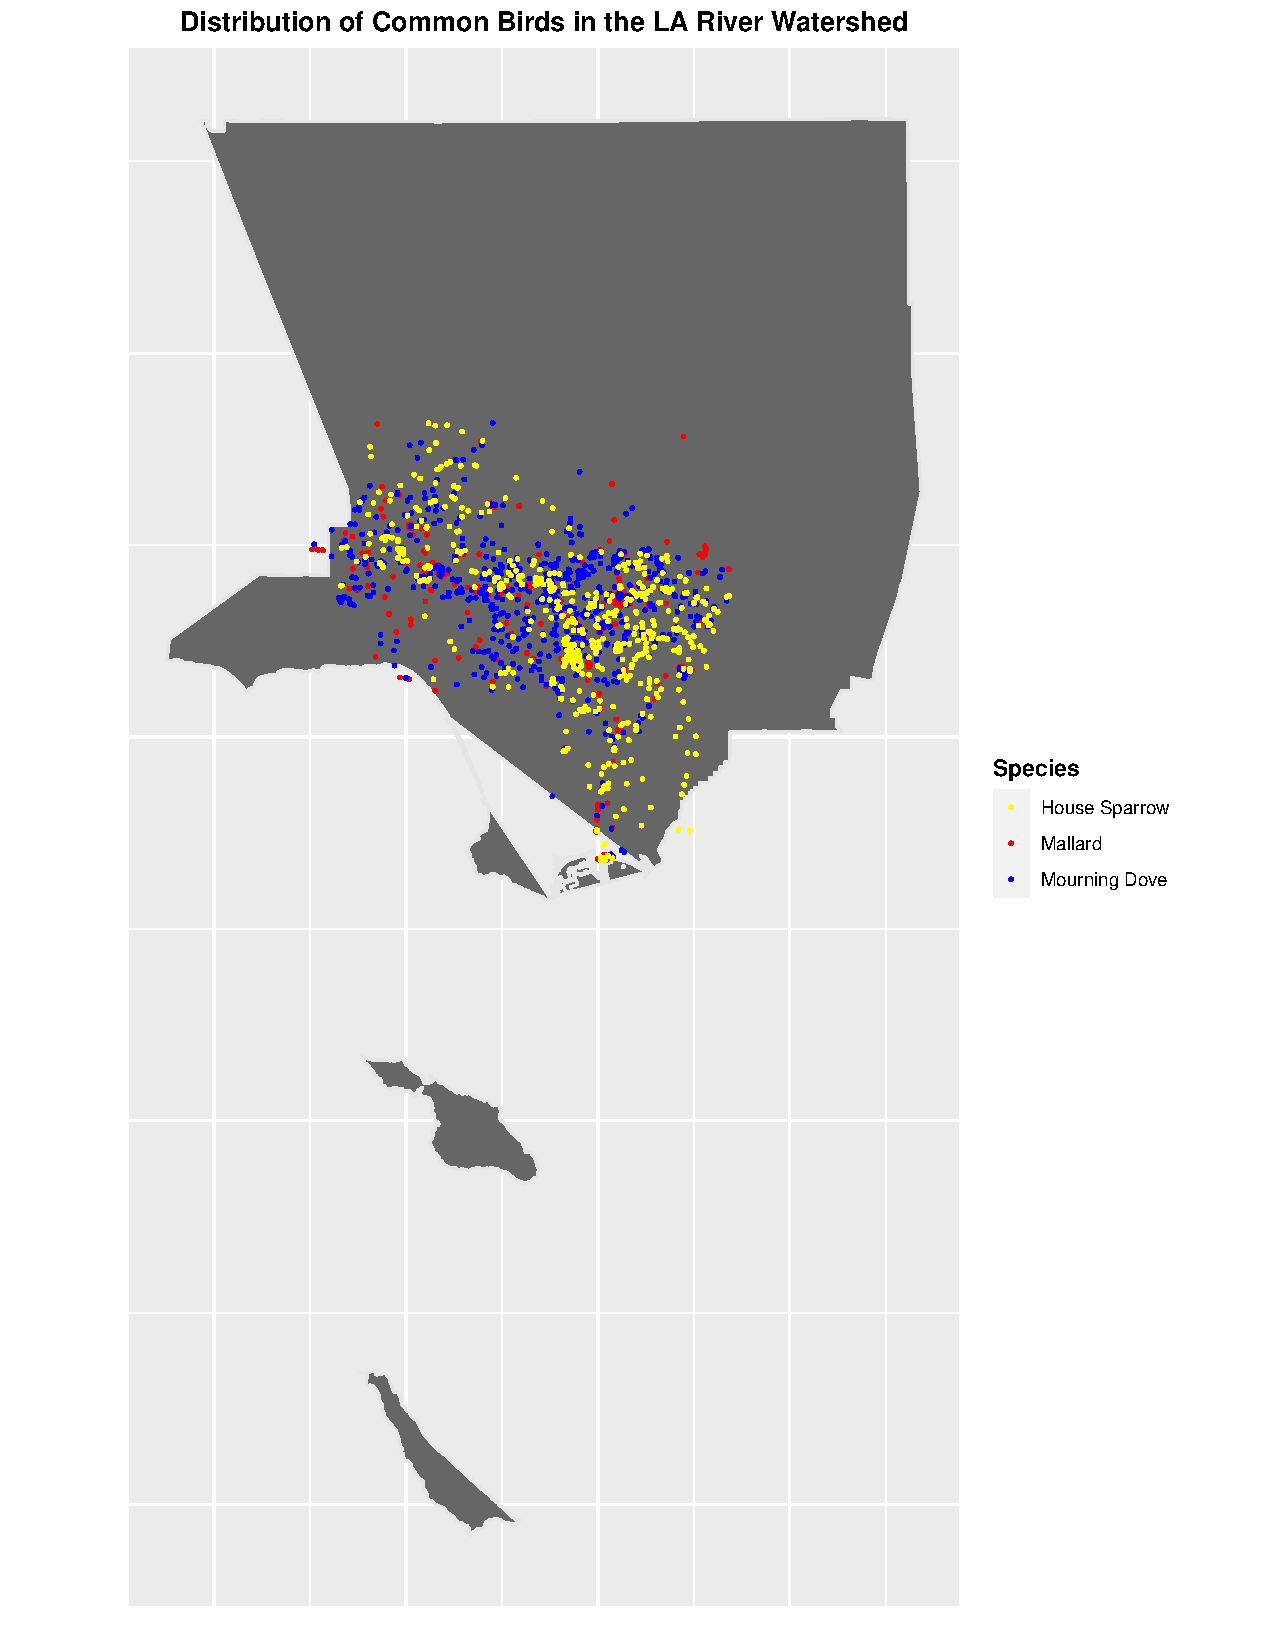
\includegraphics[width=0.45\paperwidth]{dist_map1}
	\caption{Distribution of common bird species within the LA River Watershed region based on iNaturalist data.\label{fig:map}}
\end{figure}

\newpage

\begin{figure}[h]
	\centering
	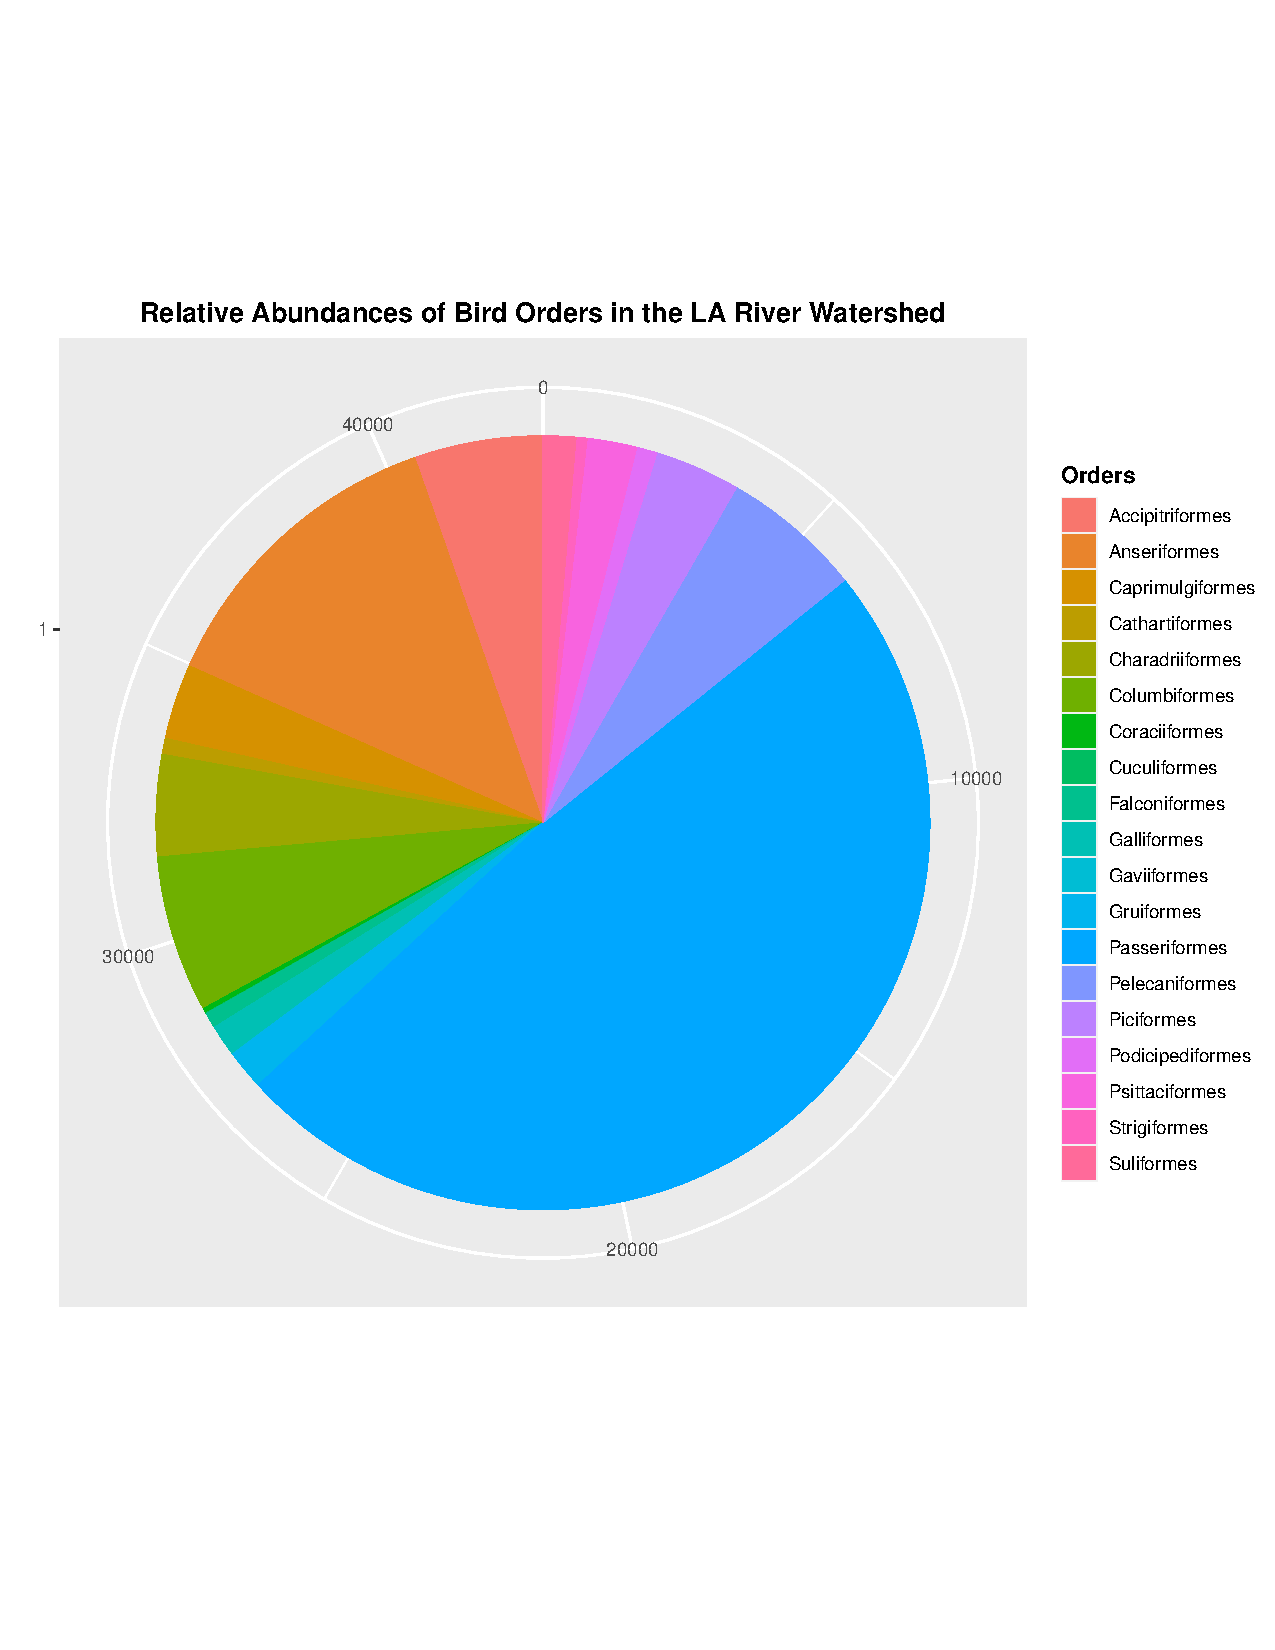
\includegraphics[width=0.6\paperwidth]{pie_chart}
	\caption{The relative abundances of bird orders within the LA River Watershed region based on iNaturalist data.\label{fig:pie}}
\end{figure}




\bibliography{references}
\bibliographystyle{plain}

\end{document}







